%-------------------------------------------------------------------------------
% LSD: a Line Segment Detector
% by Rafael Grompone von Gioi, Jeremie Jakubowicz,
%    Jean-Michel Morel & Gregory Randall
% IPOL 2012
%-------------------------------------------------------------------------------
\documentclass{ipol}
\ipolSetYear{2012}
\ipolSetDOI{10.XXXX/ipol.2012.gjmr-lsd}

\usepackage{hyperref,verbatim,graphicx,amsmath,amssymb,amssymb,dsfont}
\usepackage[ruled,linesnumbered]{algorithm2e}
\newtheorem{theorem}{Theorem}
\begin{document}

%-------------------------------------------------------------------------------
\title{LSD: a Line Segment Detector}
\author{Rafael Grompone von Gioi, J\'er\'emie Jakubowicz,\\
        Jean-Michel Morel, Gregory Randall}
\date{}
\ipolMaketitle

%-------------------------------------------------------------------------------
\begin{ipolAbstract}
LSD is a linear-time Line Segment Detector giving subpixel accurate
results. It is designed to work on any digital image without parameter
tuning. It controls its own number of false detections: On average,
one false alarms is allowed per image \cite{lsd}. The method is based
on Burns, Hanson, and Riseman method \cite{burns}, and uses an \emph{a
  contrario} validation approach according to the Desolneux, Moisan,
and Morel theory \cite{dmm2000,dmm2008}. The version described here
includes some further improvement over the one described in
\cite{lsd}.
\end{ipolAbstract}

%-------------------------------------------------------------------------------
\begin{ipolCode}
The ANSI C implementation of LSD,
\href{http://www.ipol.im/pub/algo/gjmr_line_segment_detector/lsd_1.6.zip}%
{version 1.6}, is the one which has been peer reviewed and accepted by
IPOL. The code documentation, including the source code, is
accessible
\href{http://www.ipol.im/pub/algo/gjmr_line_segment_detector/doc}{here}.
\end{ipolCode}

%-------------------------------------------------------------------------------
\begin{ipolSupp}
An older version, based on
the \href{http://megawave.cmla.ens-cachan.fr/}{Megawave2} framework is
available
\href{http://www.ipol.im/pub/algo/gjmr_line_segment_detector/lsd.zip}{here}
(this version corresponds better to the algorithm described
in \cite{lsd}, and does not include the further improvements described
here and included in the current version). This version, as the
previous
\href{http://www.ipol.im/pub/algo/gjmr_line_segment_detector/lsd-1.5.zip}{%
version 1.5}, are non reviewed
material. (Note that the interface changed from version 1.5 to version
1.6.)
\end{ipolSupp}

%-------------------------------------------------------------------------------
\section{Introduction}

LSD is aimed at detecting locally straight contours on images. This is
what we call \emph{line segments}. Contours are zones of the image
where the gray level is changing fast enough from dark to light or the
opposite. Thus, the gradient and level-lines of the image are key
concepts and are illustrated on the following figure:

\begin{center}
\includegraphics[scale=0.7]{images/edge-level-line.png}
\end{center}

The algorithm starts by computing the level-line angle at each pixel
to produce a \emph{level-line field}, i.e., a unit vector field such
that all vectors are tangent to the level line going through their
base point. Then, this field is segmented into connected regions of
pixels that share the same level-line angle up to a certain tolerance
$\tau$. These connected regions are called \emph{line support
regions}:

\begin{center}
\includegraphics[scale=0.7]{images/level-line-fields.png}
\end{center}

Each \emph{line support region} (a set of pixels) is a candidate for a
\emph{line segment}. But the corresponding geometrical object (a rectangle
in this case) must be associated with it. The principal inertial axis
of the \emph{line support region} is used as main rectangle direction; the
size of the rectangle is chosen to cover the full region:

\begin{center}
\includegraphics[height=0.3\textwidth]{images/image2.png}
\includegraphics[height=0.3\textwidth]{images/line-support-region2.png}
\includegraphics[height=0.3\textwidth]%
                {images/line-suppor-region-and-rectangle.png}
\end{center}

Each rectangle is subject to a validation procedure. The pixels in the
rectangle whose level-line angle corresponds to the angle of the
rectangle up to a tolerance $\tau$ are called \emph{aligned points}. The
total number of pixels in the rectangle, $n$, and its
number of \emph{aligned points}, $k$, are counted and used
to validate or not the rectangle as a detected \emph{line segment}.

\begin{center}
\includegraphics[scale=0.7]{images/level-line-field-rectangle.png}
\includegraphics[scale=0.7]{images/rectangle-aligned-points3.png}
\end{center}

The validation step is based on the \emph{a contrario} approach and
the Helmholtz principle proposed by Desolneux, Moisan, and Morel
\cite{dmm2000,dmm2008}. The so-called Helmholtz principle states
that no perception (or detection) should be produced on an image of
noise. Accordingly, the \emph{a contrario} approach proposes to define
a \emph{noise} or \emph{a contrario} model $H_0$ where the desired
structure is not present. Then, an event is validated if the expected
number of events as good as the observed one is small on the \emph{a
contrario} model. In other words, structured events are defined as
being rare in the \emph{a contrario} model.

In the case of \emph{line segments}, we are interested in the number
of \emph{aligned points}. We consider the event that a \emph{line
segment} in the \emph{a contrario} model has as many or more aligned
points, as in the observed \emph{line segment}. Given an image $i$ and
a rectangle $r$, we will note $k(r,i)$ the number of \emph{aligned
points} and $n(r)$ the total number of pixels in $r$. Then, the
expected number of events which are as good as the observed one is
\begin{equation}
   N_{test} \cdot P_{H_0}[k(r,I)\geq k(r,i)]
\end{equation}
where the \emph{number of tests} $N_{test}$ is the total number of
possible rectangles being considered, $P_{H_0}$ is the probability on
the \emph{a contrario} model $H_0$ (that is defined below), and $I$ is
a random image following $H_0$. The $H_0$ stochastic model fixes the
distribution of the number of aligned points $k(r,I)$, which only
depends on the distribution of the level-line field associated with
$I$. Thus $H_0$ is a noise model for the image gradient orientation
rather than a noise model for the image.

Note that $k(r,I)$ is an abuse of notation as $I$ does not corresponds
to an image but to a \emph{level-line field} following
$H_0$. Nevertheless, there is no contradiction as $k(r,I)$ only
depends on the gradient orientations.

The \emph{a contrario} model $H_0$ used for \emph{line segment}
detection is therefore defined as a stochastic model of the
\emph{level-line field} satisfying the following properties:
\begin{itemize}

  \item $\{LLA(j)\}_{j\in\textrm{Pixels}}$ is composed of independent
    random variables

  \item $LLA(j)$ is uniformly distributed over $[0,2\pi]$

\end{itemize}
where $LLA(j)$ is the level-line angle at pixel $j$. Under hypothesis
$H_0$, the probability that a pixel on the \emph{a contrario} model is
an \emph{aligned point} is
$$
   p=\frac{\tau}{\pi}
$$
and, as a consequence of the independence of the random variables
$LLA(j)$, $k(r,I)$ follows a binomial distribution. Thus, the
probability term $P_{H_0}[k(r,I)\geq k(r,i)]$ is given by
$$
   P_{H_0}\big[k(r,I) \geq k(r,i) \big] = B\big(n(r),k(r,i),p\big)
$$
where $B(n,k,p)$ is the tail of the binomial distribution:
$$
   B(n,k,p) = \sum_{j=k}^n \binom{n}{j}p^{j}(1-p)^{n-j}.
$$
The \emph{number of tests} $N_{test}$ corresponds to the total number
of rectangles that could show an alignment at a fixed
precision. Notice that the rectangles are \emph{oriented}, meaning
that the order of their starting and ending points is not arbitrary:
it encodes which side of the \emph{line segment} is darker. Thus, a
rectangle from point A to point B is a different test from the
rectangle from point B to point A. The exhaustive choice is to take
all the rectangles starting and ending at image pixels. In a $N\times
M$ image this gives $NM\times NM$ different rectangles. Also,
$\sqrt{NM}$ different width values are considered for each one.

\begin{center}
\includegraphics[scale=0.7]{images/number-of-tests.png}
\end{center}

The number of rectangles considered is then
$$
   (NM)^{5/2}.
$$
The \emph{precision} $p$ is initially set to the value $\tau/\pi$; but
other values are also tested to cover the relevant range of values;
this is explained in the section ``Rectangle Improvement''. We will
note $\gamma$ the number different $p$ values potentially tried. Each
rectangle with each $p$ value is a different test. Thus, the
final \emph{number of tests} is
$$
   (NM)^{5/2}\gamma.
$$
Finally, we define the Number of False Alarms (NFA) associated with a
rectangle $r$ on the image $i$ as
$$
   \textrm{NFA}(r,i) = (NM)^{5/2}\gamma\cdot b\Big(n(r),k(r,i),p\Big).
$$
This corresponds to the expected number of rectangles which have a
sufficient number of \emph{aligned points} to be as rare as $r$ under
$H_0$. When the NFA associated with an image rectangle is large, this
means that such an event is expected on the \emph{a contrario} model,
i.e., common and thus not a relevant one. On the other hand, when the
NFA value is small, the event is rare and probably a meaningful one. A
threshold $\varepsilon$ is selected and rectangles with
$NFA(r,i)\leq\varepsilon$ are called \emph{$\varepsilon$-meaningful
rectangles} and are the detections of the algorithm.

\begin{theorem}
$$
   E_{H_0}\left[\sum_{r\in\mathcal{R}} \mathds{1}_{\textrm{NFA}(r,I)<\varepsilon}
         \right] \leq \varepsilon
$$
where $E$ is the expectation operator, $\mathds{1}$ is the indicator
function, $\mathcal{R}$ is the set of rectangles considered, and $I$
is a random image on $H_0$.
\end{theorem}

The theorem states that the average number
of \emph{$\varepsilon$-meaningful rectangles} under the \emph{a
contrario} model $H_0$ is less than $\varepsilon$. Thus, the number of
detections on noise is controlled by $\varepsilon$ and it can be made
as small as desired. In other words, this shows that LSD satisfies the
Helmholtz principle.

The proof is given here because it was not given in the original
article \cite{lsd}.

\paragraph{Proof}
We define $\hat{k}(r)$ as
$$
   \hat{k}(r) = \min\left\{n\in\mathds{N},
                \,\,P_{H_0}\big[k(r,I)\geq n\big]
                \leq\frac{\varepsilon}{(NM)^{5/2}\gamma}\right\}.
$$
Then, $\textrm{NFA}(r,i)\leq\varepsilon$ is equivalent to
$k(r,i)\geq\hat{k}(r)$. Now,
$$
   E_{H_0}\left[\sum_{r\in\mathcal{R}}
                \mathds{1}_{\textrm{NFA}(r,I)\leq\varepsilon}\right]
                = \sum_{r\in\mathcal{R}}
                P_{H_0}\big[\textrm{NFA}(r,I)\leq\varepsilon\big] =
                \sum_{r\in\mathcal{R}}
                P_{H_0}\left[k(r,I)\geq\hat{k}(r)\right].
$$
But, by definition of $\hat{k}(r)$ we know that
$$
   P_{H_0}\left[k(r,I)\geq\hat{k}(r)\right] \leq
     \frac{\varepsilon}{(NM)^{5/2}\gamma}.
$$
and using that $\#\mathcal{R}=(NM)^{5/2}\gamma$ we get
$$
   E_{H_0}\left[\sum_{r\in\mathcal{R}}
                \mathds{1}_{\textrm{NFA}(r,I)\leq\varepsilon}\right]
                \leq \sum_{r\in\mathcal{R}} \frac{\varepsilon}{(NM)^{5/2}\gamma}
                = \varepsilon
$$
which concludes the proof.\hfill$\Box$

\medskip

Following Desolneux, Moisan, and Morel \cite{dmm2000,dmm2008}, we set
$\varepsilon=1$ once for all. This corresponds to accepting on average
one false detection per image in the \emph{a contrario} model, which
is reasonable. Also, the detection result is not sensitive to the
value of $\varepsilon$. Indeed, the detection limit (that is the
minimal number of aligned points that could lead to
a \emph{$\varepsilon$-meaningful rectangle}) varies like
$\sqrt{-\log\varepsilon}$. Setting $\varepsilon$ to any reasonable
value would produce very similar results.

%-------------------------------------------------------------------------------
\section{Algorithm}

The LSD algorithm takes a gray-level image as input and returns a list
of detected \emph{line segments}. The algorithm can be described by
the following 12 steps that will be described in detail below. The
auxiliary image STATUS has the same size as the scaled image, and is
used to keep track of the pixels already used.

\begin{algorithm}
Scale the input image to scale S using Gaussian sub-sampling
  ($\sigma=\frac{\Sigma}{S}$).\;
Compute the gradient magnitude and level-line orientation at each pixel.\;
Build a list of pixels pseudo-ordered according to their
  image gradient magnitude.\;
Set all pixels in the auxiliary image STATUS to the value NOT USED.\;
Mark the STATUS of pixels whose gradient magnitude is less than
  $\rho$ to the value USED.\;
\ForEach{pixel P in the list, starting with the ones with the
  highest gradient magnitude, and with STATUS set to NOT USED}
  {
    Starting from P as a seed pixel, grow a region R of connected
      and NOT USED pixels, that share the same level-line angle
      up to a tolerance $\tau$. Mark the STATUS of the pixels
      in the region as USED.\;
    Compute the rectangular approximation for the connected region R
      of pixels found.\;
    If the density of aligned points in the rectangle is less than D,
      cut the region, until the density restriction is satisfied.\;
    Compute the NFA value for the rectangle found.\;
    Try to modify the rectangle to improve the NFA value.\;
    If $\textrm{NFA}(r) \leq \varepsilon$,
      add the rectangle to the output list.\;
  }
\end{algorithm}

LSD was designed as an automatic image analysis tool. As such it must
work without requiring any parameter tuning. The algorithm actually
depends on several numbers that determine its behavior; their values
were carefully devised to work on all images. (See their discussion
below.) They are therefore part of LSD's design, internal parameters,
and are not left to the user's choice. Changing their values would
amount to define a new variant of the algorithm, in the same way as we
could make variants by changing the gradient operator, or by switching
from 8-neighborhood to 4-neighborhood on the region growing process.

Each step of the algorithm will be described in the following
sections, as well as the design criteria for setting the six internal
parameters: S, $\Sigma$, $\rho$, $\tau$, D, and
$\varepsilon$.

%[The algorithm main function in LSD code is
%[`LineSegmentDetection`](doc/lsd_8c.html#a54).]

%-------------------------------------------------------------------------------
\subsection{Image scaling}

The result of LSD is different when the image is analyzed at different
scales or if the algorithm is applied to a small part of the
image. This is natural, and corresponds to the different details that
one can see if an image is observed from a distance or if attention is
paid to a specific part. As a result of the \emph{a contrario}
validation step, the detections thresholds automatically adapt to the
image size that is directly related to the number of tests term. The
scale of analysis is a choice left to the the user, who can select it
by cropping the image. Otherwise LSD processes automatically the
entire image.

The first step of LSD is, nevertheless, to scale the input image to
80\% of its size. This scaling helps to cope with aliasing and
quantization artifacts (especially the staircase effect) present in
many images. Blurring the image would produce the same effect but
affecting statistics of an image in the \emph{a contrario} model: some
structures would be detected on a blurred white noise. When correctly
sub-sampled, the white noise statistics are preserved. Note that the
\emph{a contrario} validation is applied to the scaled image and the
$N\times M$ image size used in the NFA computation corresponds to an
input image of size $1.25N\times 1.25M$.

The following images show two discrete edges at different angles, both
presenting the staircase effect. Next to each image is the result of
LSD without using the initial scaling. In the first case the edge is
detected as four horizontal line segments instead of one; in the
second case, no line segment is detected:

\begin{center}
\includegraphics[scale=0.7]{images/edge0.png}
\includegraphics[scale=0.7]{images/edge0_lsd-s1.png}
\includegraphics[scale=0.7]{images/edge1.png}
\includegraphics[scale=0.7]{images/edge1_lsd-s1.png}
\end{center}

In both cases the result is reasonable, but it does not correspond to
what we would expected. The following figures show the result of LSD,
using the 80\% scaling. Both edges are now detected and with the right
orientation (even if the first one is still fragmented).

\begin{center}
\includegraphics[scale=0.7]{images/edge0_lsd.png}
\includegraphics[scale=0.7]{images/edge1_lsd.png}
\end{center}

The scale factor of 80\% (S=0.8), is the smallest image reduction that
reasonably solves the staircase problem while producing almost the
same result as a full scale analysis on images without artifacts. (A
80\% scaling means here that the x and y axis are each reduced to
80\%; the number of pixels is thus reduced to 64\%.)

The scaling is performed by a Gaussian sub-sampling: the image is
filtered with a Gaussian kernel to avoid aliasing and then
sub-sampled. The standard deviation of the Gaussian kernel is
determined by $\sigma=\Sigma/S$, where S is the scaling factor. The
value of $\Sigma$ is set to 0.6, which gives a good balance between
avoiding aliasing and avoiding image blurring.

%[The scaling is performed in LSD code by the function
%[`gaussian_sampler`](doc/lsd_8c.html#a32).]

%-------------------------------------------------------------------------------
\subsection{Gradient computation}

The image gradient is computed at each pixel using a 2x2 mask. Given
$$
   \begin{array}{c|c|c|c}
                  \ddots & \vdots   & \vdots     & \cdots \\
                  \hline
                  \cdots & i(x,y)   & i(x+1,y)   & \cdots \\
                  \hline
                  \cdots & i(x,y+1) & i(x+1,y+1) & \cdots \\
                  \hline
                  \cdots & \vdots   & \vdots     & \ddots \\
                \end{array}
$$
where $i(x,y)$ is the image gray level value at pixel
$(x,y)$, the image gradient is computed as
$$
   g_x(x,y)=\frac{i(x+1,y)+i(x+1,y+1)-i(x,y)-i(x,y+1)}{2},
$$
$$
   g_y(x,y)=\frac{i(x,y+1)+i(x+1,y+1)-i(x,y)-i(x+1,y)}{2}.
$$
The level-line angle is computed as
$$
   \arctan{\left(\frac{g_x(x,y)}{-g_y(x,y)}\right)}
$$
and the gradient magnitude as
$$
   G(x,y)=\sqrt{ g_x^2(x,y) + g_y^2(x,y) }.
$$
This simple scheme uses the smallest possible mask size in its
computation, thus reducing as much as possible the dependence of the
computed gradient values (thus, approaching the theoretical
independence in the case of a noise image).

The gradient and level-line angles encode the direction of the edge,
that is, the angle of the dark to light transition. Note that a dark
to light transition and a light to dark transition are different,
having a 180 degree angle difference between the corresponding
gradient or level-line angles. This means that the
resulting \emph{line segments} detected by LSD are oriented and that
the order of their starting and ending points is not arbitrary, since
it encodes which side of the \emph{line segment} is darker. For
example, if the contrast of an image is reverted (changing black for
white and white for black) the result of LSD would be the same but the
starting and ending points would be exchanged on every \emph{line
segment}.

Note that the computed value corresponds to the image gradient at
coordinates $(x+0.5,y+0.5)$ and not $(x,y)$. This half-pixel offset is
then added to the output rectangles coordinates to produce coherent
results.

In the \emph{a contrario} model, the \emph{level-line field} is
composed of independent random variables at each pixel. But the
computed \emph{level-line field} is actually never fully independent
even if the image is a white noise. Indeed, adjacent pixel values are
used to compute the gradient and therefore the gradients are
(slightly) dependent. This does not prevent the use of an \emph{a
contrario} approach. Indeed, numerical simulations have shown that the
same threshold deduced for the case of independent \emph{level-line
field} also controls the number of false detections when computed by
the 2x2 mask, see \cite{multiseg}.

%[In the LSD code, the gradient computation, gradient threshold, and
%pseudo-ordering, are all performed by the function
%[`ll_angle`](doc/lsd_8c.html#a33).]

%-------------------------------------------------------------------------------
\subsection{Gradient Pseudo-ordering}

LSD is a greedy algorithm and the order in which pixels are processed
has an impact on the result. Pixels with high gradient magnitude
correspond to the more contrasted edges. In an edge, the central
pixels usually have the highest gradient magnitude. So it makes sense
to start looking for \emph{line segments} at pixels with the highest
gradient magnitude.

Sorting algorithms usually require $O(n\log n)$ operations to sort $n$
values. However, a simple pixel pseudo-ordering is possible in
linear-time. To this aim, 1024 bins are created corresponding to equal
gradient magnitude intervals between zero and the largest observed
value on the image. Pixels are classified into the bins according to
its gradient magnitude. LSD uses first seed pixels from the bin of the
largest gradient magnitudes; then it takes seed pixels from the second
bin, and so on until exhaustion of all bins. 1024 bins are enough to
sort almost strictly the gradient values when the gray level values
are quantized in the integer range [0,255].

%[In the LSD code, the gradient computation, gradient threshold, and
%pseudo-ordering, are all performed by the function
%[`ll_angle`](doc/lsd_8c.html#a33).]

%-------------------------------------------------------------------------------
\subsection{Gradient threshold}

Pixels with small gradient magnitude correspond to flat zones or slow
gradients. Also, they naturally present a higher error in the gradient
computation due to the quantization of their values. In LSD the pixels
with gradient magnitude smaller than $\rho$ are therefore rejected and
not used in the construction of \emph{line-support regions} or
rectangles.

Assuming a quantization noise $n$ and an ideal image $i$ we observe:
$$
   \tilde{i} = i + n \qquad \nabla\tilde{i} = \nabla i + \nabla n.
$$

\begin{center}
\includegraphics[scale=0.7]{images/angle-error.png}
\end{center}

We have
$$
   |\textrm{angle error}| \leq \arcsin\left(\frac{q}{|\nabla i|}\right),
$$
where $q$ is a bound on $|\nabla n|$. The criterion used is to reject
pixels where the angle error is larger than the angle tolerance $\tau$
used in the region growing algorithm. That is, we impose
$|\textrm{angle error}|\leq\tau$ and we get
$$
   \rho = \frac{q}{\sin{\tau}}.
$$
The threshold $\rho$ is set using the last expression where $q$ is a
bound on the possible error in the gradient value due to quantization
effects \cite{lsd}, and $\tau$ is the angle tolerance to be used in
the region growing algorithm.

In the usual case, the pixel values are quantized to integer values in
$\{0,1,\dots,255\}$. Thus, the maximal possible error in the gradient
is 2 (when adjacent pixels have quantization errors of one that do not
compensate). Thus, we set $q=2$.  This value will not, however, give
good results if the image intensity range differs significantly from
the [0,255] interval.

%[In the LSD code, the gradient computation, gradient threshold, and
%pseudo-ordering, are all performed by the function
%[`ll_angle`](doc/lsd_8c.html#a33).]

%-------------------------------------------------------------------------------
\subsection{Region Growing}

Starting from a pixel in the ordered list of unused pixels, the seed,
a region growing algorithm is applied to form a \emph{line-support
region}.  Recursively, the unused neighbors of the pixels already in
the region are tested, and the ones whose level-line angle is equal to
the \emph{region angle} $\theta_{region}$ up to a tolerance $\tau$ are
added to the region. The initial \emph{region angle} $\theta_{region}$
is the level-line angle of the seed point, and each time a pixel is
added to the region the \emph{region angle} value is updated to
$$
   \arctan\left(\frac{\sum_j \sin(\textrm{level-line-angle}_j)}
                       {\sum_j \cos(\textrm{level-line-angle}_j)}\right)
$$
where the index $j$ runs over the pixels in the region. If we
associate to each pixel in the region a unitary vector with its
level-line angle, the latter formula corresponds to the angle of the
mean vector. The process is repeated until no other pixel can be added
to the region. The following pseudo-code gives a precise definition:

\begin{algorithm}
The initial point $P$ is added to the Region $\theta_{region}$ is set
  to the level-line angle of pixel $P$\;
$S_x\leftarrow\cos(\theta_{region})$\;
$S_y\leftarrow\sin(\theta_{region})$\;
\ForEach{For each pixel $P$ in the Region}
  {
    \ForEach{pixel $Q$ neighbor of $P$
             and $\textrm{Status}(Q)\neq\textrm{USED}$}
      {
        \If{$\textrm{AngleDifference}\left(\theta_{region},
                       \textrm{level-line-angle}(Q)\right)<\tau$}
          {
            Add $Q$ to the Region\;
            $\textrm{Status}(Q)\leftarrow\textrm{USED}$\;
            $S_x \leftarrow S_x+\cos(\textrm{LevelLineAngle}(Q))$\;
            $S_y \leftarrow S_y+\sin(\textrm{LevelLineAngle}(Q))$\;
            $\theta_{region} \leftarrow \arctan(S_y/S_x)$\;
          }
      }
  }
\end{algorithm}

An 8-connected neighborhood is used, so the neighbors of pixel
$i(x,y)$ are $i(x-1,y-1)$, $i(x,y-1)$, $i(x+1,y-1)$, $i(x-1,y)$,
$i(x+1,y)$, $i(x-1,y+1)$, $i(x,y+1)$, and $i(x+1,y+1)$.

The tolerance $\tau$ is set to 22.5 degree or $\pi/8$ radian, that
corresponds to a 45 degree range or $1/8$ of the full range of
orientations. It was chosen because it is near the largest possible
value that still makes sense to call a pixel "oriented like the
rectangle". What is important is not the exact value but the order of
magnitude, so it was set to obtain $p=1/8$. The next figure shows a
typical example. On the left we see a detail of a noisy edge. Next to
it is the result of the region growing algorithm for $\tau$ set to
11.25, 22.5, and 45 degree, respectively. The first case is too
restrictive and the region is too small; with 45 degree regions often
expand too far from the edge; 22.5 is a good compromise.

\begin{center}
\includegraphics[scale=0.5]{images/region_img_x.png}
\includegraphics[scale=0.5]{images/region11_25x.png}
\includegraphics[scale=0.5]{images/region22_5x.png}
\includegraphics[scale=0.5]{images/region45x.png}
\end{center}

Regions that could be obtained with a smaller value are also obtained
in this way. In the validation process, smaller values of the
precision $p$ are also tested, so the value of $\tau$ only affects the
region growing algorithm and not the validation.

%[The region growing step is done in the LSD code by the function
%[`region_grow`](doc/lsd_8c.html#a50).]

%-------------------------------------------------------------------------------
\subsection{Rectangular Approximation}

A \emph{line segment} corresponds to a geometrical event, a rectangle.
Before evaluating a \emph{line-support region}, the rectangle
associated with it must be found. The region of pixels is interpreted
as a solid object and the gradient magnitude of each pixel is used as
the ``mass'' of that point. Then, the center of mass of the region is
selected as the center of the rectangle and the main direction of the
rectangle is set to the first inertia axis of the region. Finally, the
width and length of the rectangles are set to the smallest values that
make the rectangle to cover the full \emph{line-support region}.

The center of the rectangle $(c_x,c_y)$ is set to
$$
   c_x = \frac{\sum_{j\in \textrm{Region}} G(j) \cdot x(j)}
                           {\sum_{j\in \textrm{Region}} G(j)}
$$
$$
   c_y = \frac{\sum_{j\in \textrm{Region}} G(j) \cdot y(j)}
                           {\sum_{j\in \textrm{Region}} G(j)}
$$
where $G(j)$ is the gradient magnitude of pixel $j$, and the index $j$
runs over the pixels in the region. The main rectangle's angle is set
to the angle of the eigenvector associated with the smallest
eigenvalue of the matrix
$$
   M = \left(\begin{array}{cc}
               m^{xx} & m^{xy} \\
               m^{xy} & m^{yy} \\
             \end{array}\right)
$$
with
$$
   m^{xx} = \frac{\sum_{j\in\textrm{Region}}G(j)\cdot(x(j)-c_x)^2}
                              {\sum_{j\in\textrm{Region}}G(j)}
$$
$$
   m^{yy} = \frac{\sum_{j\in\textrm{Region}}G(j)\cdot(y(j)-c_y)^2}
                              {\sum_{j\in\textrm{Region}}G(j)}
$$
$$
   m^{xy} = \frac{\sum_{j\in\textrm{Region}}G(j)\cdot
                (x(j)-c_x)(y(j)-c_y)}{\sum_{j\in\textrm{Region}}G(j)}.
$$

%[In the LSD code, the rectangular approximation is computed by the
%function [`region2rect`](doc/lsd_8c.html#a49), using the function
%[`get_theta`](doc/lsd_8c.html#a48) to compute the main rectangle's
%angle.]

%-------------------------------------------------------------------------------
\subsection{NFA Computation}

A key concept in the validation of a rectangle is that
of \emph{$p$-aligned points}, namely the pixels in the rectangle whose
level-line angle is equal to the rectangle's main orientation, up to a
tolerance $p\pi$. The \emph{precision} $p$ is initially set to the
value $\tau/\pi$, but other values are also tested as is explain in
the section "Rectangle Improvement"; a total of $\gamma$ different
values for $p$ are tried. The total number of pixels in the rectangle
is denoted by $n$ and the number of \emph{$p$-aligned points} is
denoted by $k$ (we drop $r$ and $i$ when they are implicit to simplify
the notation). Then, the number of false alarms (NFA) associated with
the rectangle $r$ is
$$
   \textrm{NFA}(r) = (NM)^{5/2}\gamma\cdot b(n,k,p)
$$
where N and M are the number of columns and rows of the image (after
scaling), and $b(n,k,p)$ is the binomial tail
$b(n,k,p)=\sum_{j=k}^{n}\binom{n}{j}p^j(1-p)^{n-j}.$

All in all, for each rectangle being evaluated and given
a \emph{precision} $p$, the numbers $k$ and $n$ are counted, and then
the NFA value is computed by
$$
   \textrm{NFA}(r) = (NM)^{5/2}\gamma \cdot
                                  \sum_{j=k}^{n}\binom{n}{j}p^j(1-p)^{n-j}.
$$
The rectangles with $\textrm{NFA}(r)\leq\varepsilon$ are validated as
detections.

As stated before, and following Desolneux, Moisan, and
Morel \cite{dmm2000,dmm2008}, we set $\varepsilon=1$ once for
all. Here we will only show an experiment illustrating the stability
of the result relative to $\varepsilon$ value. Below is the input
image and the result of LSD with $\varepsilon=1$,
$\varepsilon=10^{-1}$, and $\varepsilon=10^{-2}$, respectively. Only a
few small line segments disappear:

\begin{center}
\includegraphics[scale=0.4]{images/office.png}
\includegraphics[scale=0.4]{images/office_lsd-e0.png}
\includegraphics[scale=0.4]{images/office_lsd-e1.png}
\includegraphics[scale=0.4]{images/office_lsd-e2.png}
\end{center}

In our implementation, the computation of the binomial tail is
performed using the the following relation to the Gamma function:
$$
   \binom{n}{k} = \frac{\Gamma(n+1)}{\Gamma(k+1)\cdot\Gamma(n-k+1)}.
$$
The Gamma function can be efficiently computed. We use the methods by
Lanczos and Windschitl as described
on \url{http://www.rskey.org/gamma.htm}. To speed up the computations,
the sum of the binomial tail is truncated when the error can be
bounded to be less than 10\%.

%[The function [`rect_nfa`](doc/lsd_8c.html#a47) of the LSD code counts
%the number of \emph{aligned points} and the total number of points, and
%then computes the NFA, calling the function
%[`nfa`](doc/lsd_8c.html#a39) to compute the binomial tail.]

%-------------------------------------------------------------------------------
\subsection{\emph{Aligned Points} Density}

In some cases, the $\tau$-angle-tolerance method produces a wrong
interpretation. This problem can arise when two straight edges are
present in the image forming an angle between them smaller than the
tolerance $\tau$. The following image shows an example of
a \emph{line-support region} found (in gray) and the rectangle
corresponding to it.

\begin{center}
\includegraphics[scale=0.7]{images/angle-problem.png}
\end{center}

This \emph{line-support region} could be better interpreted as two
thinner rectangles, one longer than the other, forming an obtuse
angle.

In LSD this problem is handled by detecting
problematic \emph{line-support regions} and cutting them into two
smaller regions, hoping to cut the region at the right place to solve
the problem. Once a cut region is accepted, the rectangle associated
is recomputed and the algorithm is resumed.

The detection of this ``angle problem'' is based on the density of
\emph{aligned points} in the rectangle. When this problem is not present,
the rectangle is well adapted to the \emph{line-support region} and
the density of \emph{aligned points} is high. On the other hand, when
the ``angle problem'' is present, as can be seen on the previous
figure, the density of \emph{aligned points} is low. Also, when a
slightly curved edge is being locally approximated by a sequence of
straight edges, the degree of the approximation (how many \emph{line
segments} are used to cover part of curve) is related to the density
of \emph{aligned points}; this means that $D$ also controls how curves
are approximated by \emph{line segments}.

The density of \emph{aligned points} of a rectangle is computed as the
ratio of the number of \emph{aligned points} ($k$ in the previous
notation) to the area of the rectangle:
$$
   d = \frac{k}{\textrm{length}(r) \cdot \textrm{width}(r)}.
$$
A threshold $D$ is defined and rectangles should have a density $d$
larger or equal to $D$ to be accepted. We set $D$ to the value 0.7
(70\%) which provides good balance between solving the ``angle
problem'', providing smooth approximations to curves, without
over-cutting the \emph{line segments}.

Two methods for cutting the region are actually tried: \emph{reduce
angle tolerance} and \emph{reduce region radius}. In both methods,
part of the pixels in the region are kept, while the others are
re-marked again as NOT USED, so they can be used again in
future \emph{line-support regions}.  We will describe now these two
methods:

%-------------------------------------------------------------------------------
\subsubsection{Reduce angle tolerance}

The first method, \emph{reduce angle tolerance}, tries to guess a new
tolerance $\tau'$ that adapts well to the region, and then the region
growing algorithm is used again with the same seed but using the newly
estimated tolerance value. When two straight regions that form an
obtuse angle are present, this method is expected to get the tolerance
that would get only one of these regions, the one containing the seed
pixel.

If all the pixels in the region were used in the estimation of the
tolerance, the new value would be such that all the pixels would still
be accepted. Instead, only the pixels near the seed are
used. Actually, only the pixels whose distance to the seed point is
less than the width of the rectangle initially computed are used. In
that way, the size of the neighborhood used in the estimation of
$\tau'$ adapts to the size of the region.

All the pixels in that neighborhood of the seed point are evaluated,
and the new tolerance $\tau'$ is set to twice the standard deviation
of the level-line angles of these pixels. With this new value, the
same region growing algorithm is applied, starting from the same seed
point. Before that, all the pixels on the original regions are set to
NOT USED, so the algorithm can use them again, and the discarded ones
are available for further regions.

%[The reduce angle tolerance method is implemented by the function
%[`refine`](doc/lsd_8c.html#a53) in the LSD code.]

%-------------------------------------------------------------------------------
\subsubsection{Reduce region radius}

The previous method, \emph{reduce angle tolerance}, is tried only
once, and if the resulting \emph{line-support region} fails to satisfy
the density criterion a second method is repetitively tried. The idea
of this second method is to gradually remove the pixels that are
farther from the seed until the criterion is satisfied or the region
is too small and rejected. This method works best when
the \emph{line-support region} corresponds to a curve and the region
needs to be reduced until the density criterion is satisfied, usually
meaning that a certain degree of approximation to the curve is
obtained.

The distance from the seed point to the farther pixel in the region is
called the \emph{radius} of the region. Each iteration of this method
removes the farthest pixels of the region to reduce the region's
\emph{radius} to 75\% of its value. This process is repeated until the
density criterion is satisfied or until there are not enough pixels in
the region to form a \emph{meaningful rectangle}. This is just a way of
gradually reducing the region until the criterion is satisfied; it
could be done one pixel at a time, but that would make the process
slower.

%[The \emph{reduce region radius} method is implemented in the
%[`reduce_region_radius`](doc/lsd_8c.html#a52) function of the LSD code.]

%-------------------------------------------------------------------------------
\subsection{Rectangle Improvement}

Before rejecting a \emph{line-support region} for being
not \emph{meaningful} ($\textrm{NFA}>\varepsilon$), LSD tries some
variations of the rectangle's configuration initially found with the
aim to get a valid one.

The relevant factors tested are the \emph{precision} $p$ used and the
width of the rectangle.

The initial \emph{precision} used, corresponding to the region growing
tolerance $\tau$ is large enough so only testing smaller values makes
sense. If the pixels are well aligned, using a finer \emph{precision}
will keep the same number of aligned points, but a smaller $p$ yields
a smaller (and therefore better) NFA.

In a similar way, it only makes sense to try to reduce the rectangle's
width because the initial width was chosen to cover the whole
\emph{line-support region}. Often, reducing by one pixel the width may
reduce the number of \emph{aligned points} by only a few units while
reducing the total number of pixels by a number equal to the length of
the rectangle, see the figure below. This may decrease significantly
the binomial tail and therefore also the NFA.

\begin{center}
\includegraphics[scale=0.7]{images/region_ex.png}
\end{center}

The \emph{rectangle improvement} routine of LSD consists of the
following steps:

1. try finer \emph{precisions}
2. try to reduce width
3. try to reduce one side of the rectangle
4. try to reduce the other side of the rectangle
5. try even finer precisions

If a \emph{meaningful rectangle} is found
($\textrm{NFA}\leq\varepsilon$) the improvement routine will stop
after the step that found it.

Step 1 tries the following \emph{precision} values: $p/2$, $p/4$,
$p/8$, $p/16$, and $p/32$, where $p$ is the initial \emph{precision}
value. The value that produces the best NFA (the smallest) value is
kept.

Step 2 tries up to five times to reduce the rectangle width by $0.5$
pixels. This means that the tested width values are $W$, $W-0.5$,
$W-1$, $W-1.5$, $W-2$, and $W-2.5$, where $W$ is the initial width
value. Again, the value that produces the best NFA value is kept.

Step 3 tries five times to reduce only one side of the rectangle by
0.5 pixel. This implies reducing the width of the rectangle by 0.5
pixels but also moving the center of the rectangle by 0.25 pixels to
maintain the position of the other side of the rectangle. So the
tested side displacements are 0.5, 1, 1.5, 2, and 2.5 pixels. As
before, the value that produces the best NFA value is kept.

Step 4 does the same thing as step 3 on the other side of the
rectangle.

Step 5 tries again to reduce the \emph{precision} still more. This
step tests the precision values $\hat{p}/2$, $\hat{p}/4$, $\hat{p}/8$,
$\hat{p}/16$, and $\hat{p}/32$, where $\hat{p}$ is
the \emph{precision} at the beginning of this step. The value that
produces the best NFA value is kept.

In addition to the initial precision $p=\frac{\tau}{\pi}$, five more
values are potentially tested in step 1 and still five more in step
5. Then $\gamma=11$. The range of precisions covered is from
$p=\frac{\tau}{\pi}$ to $p=\frac{\tau}{1024\pi}$ and is more than
enough to consider any relevant case, the finer precision being about
0.02 degree. Five such steps, attaining a 1 degree precision, would be
enough; this refinement, however, works better sometimes before and
sometimes after the width refinement, and there is no serious caveat
in performing both.

%[The rectangle improvement routine is performed by the function
%[`rect_improve`](doc/lsd_8c.html#a51) of LSD code.]

%-------------------------------------------------------------------------------
\subsection{Computational complexity}

Performing a Gaussian sub-sampling and computing the image gradient,
both can be performed with a number of operations proportional to the
number of pixels in the image. Then, pixels are pseudo-ordered by a
classification into bins, operation that can be done in linear
time. The computational time of the line-support region finding
algorithm is proportional to the number of visited pixels, and this
number is equal to the total number of pixels in the regions plus the
border pixels of each one. Thus, the number of visited pixels remains
proportional to the total number of pixels of the image. The rest of
the processing can be divided into two kind of tasks. The first kind,
for example summing the region mass or counting aligned points, are
proportional to the total number of pixels involved in all
regions. The second kind, like computing inertia moments or computing
the NFA value from the number of aligned points, are proportional to
the number of regions. Both the total number of pixels involved and
the number of regions are at most equal to the number of pixels. All
in all, LSD has an execution time proportional to the number of pixels
in the image.

%-------------------------------------------------------------------------------
\section{Examples}

The following set of examples tries to give an idea of the kind of
results obtained with LSD, both good and bad.

\paragraph{chairs:} A good result. The detected \emph{line segments}
correspond to empirically straight structures in the image. The
detection corresponds roughly with the perceptually expected result.

\begin{center}
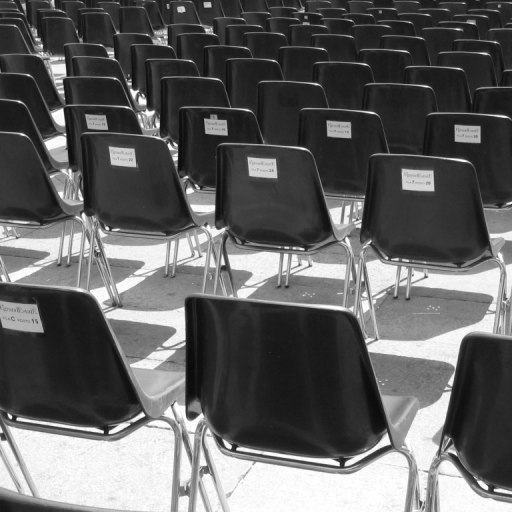
\includegraphics[scale=0.4]{images/chairs.png}
\includegraphics[scale=0.4]{images/chairs_lsd.png}
\end{center}

\paragraph{molecule-lsd:} Note that LSD detects locally
straight \emph{edges}, so each black stroke produces \emph{two}
detections, one for each white to black transition. Also note that
there is a minimal length that a line segment must have, and smaller
ones cannot be detected. (For example, the base of the number '2'.)
This minimal size for detection depends on the image size because the
NFA increases with the image size.

\begin{center}
\includegraphics[scale=0.7]{images/molecule-lsd.png}
\includegraphics[scale=0.7]{images/molecule-lsd_lsd.png}
\end{center}

\paragraph{circles:} Note that when curves are present, LSD produces
short line segments corresponding to curve sections that are locally
straight. The result is a polygonal approximation for curves. When the
curvature is too strong LSD of course fails.

\begin{center}
\includegraphics[scale=0.7]{images/circles.png}
\includegraphics[scale=0.7]{images/circles_lsd.png}
\end{center}

\paragraph{noise:} LSD was designed to provide a good false detection
control. Its false detection control is based on automatically
providing detections thresholds that prevent detections that could
happen by chance on images of noise.

\begin{center}
\includegraphics[scale=0.7]{images/noise.png}
\includegraphics[scale=0.7]{images/noise_lsd.png}
\end{center}

\paragraph{shadow and noise:} A significant part of the visible straight
structure in the following image is not detected. The reasons are the
slow gradient in the shadow and the presence of noise. However, the
structure can be detected by LSD at a different scale as is shown on
the next example.

\begin{center}
\includegraphics[scale=0.7]{images/shadow-noise.png}
\includegraphics[scale=0.7]{images/shadow-noise_lsd.png}
\end{center}

\paragraph{shadow and noise, subsampling:} When a Gaussian sub-sampling
is applied to the previous image, the noise is partially removed and
the structure is analyzed at the right scale. The expected line
segments are detected.

\begin{center}
\includegraphics[scale=0.7]{images/shadow-noise_half.png}
\includegraphics[scale=0.7]{images/shadow-noise_half_lsd.png}
\end{center}

\paragraph{small:} Due to the \emph{a contrario} framework used
by LSD to control the number of false detection, the result depends on
the image size: the number of tests depends on it. As a consequence,
the result of LSD may be locally different if the algorithm is applied
to the full image or to a crop of it. The following image contains a
little square just under the detection limit. No detection is thus
produced. The next example, however, shows a crop of this same image
and the square is indeed detected. This is the natural behavior of LSD
and means that the detail level depends on the size of the whole data
being analyzed. Human perception is similar: small details often go
unnoticed unless attention is drawn to them.

\begin{center}
\includegraphics[scale=0.7]{images/little.png}
\includegraphics[scale=0.7]{images/little_lsd.png}
\end{center}

\paragraph{small, crop:} A crop of the previous example, centered on
the square. The square is now detected.

\begin{center}
\includegraphics[scale=0.7]{images/little_crop.png}
\includegraphics[scale=0.7]{images/little_crop_lsd.png}
\end{center}

\paragraph{sky:} Some regions are partially anisotropic and partially
straight. Such regions can produce unexpected detections.

\begin{center}
\includegraphics[scale=0.7]{images/sky.png}
\includegraphics[scale=0.7]{images/sky_lsd.png}
\end{center}

\paragraph{gibbs:} Image compression, Gibbs effects are responsible
for many unexpected detections.

\begin{center}
\includegraphics[width=0.3\textwidth]{images/gibbs.png}
\includegraphics[width=0.3\textwidth]{images/gibbs_lsd.png}
\end{center}

\paragraph{color:} LSD is designed to work on gray-level images.
Before applying LSD to a color image it must be converted to a
gray-level image. However, some color edges could be lost in this
conversion.  For example, the following image presents a clear edge
(left), but after the standard conversion to a gray-level image
(middle) the edge is lost. The reason is that the red value and the
green value are both converted to the same gray value. Thus, LSD will
produce no detection (right) because \emph{none is present} in the
input image to LSD (middle). The edge is lost on the color to gray
image conversion and not by LSD. An extension of LSD to deal with this
(relatively rare) event is possible but was not done in the current
implementation.

\begin{center}
\includegraphics[width=0.3\textwidth]{images/color-step.png}
\includegraphics[width=0.3\textwidth]{images/color-step_bw.png}
\includegraphics[width=0.3\textwidth]{images/color-step_lsd.png}
\end{center}

\paragraph{real world scene:} All in all, LSD usually produces a
reasonable result on real images.

\begin{center}
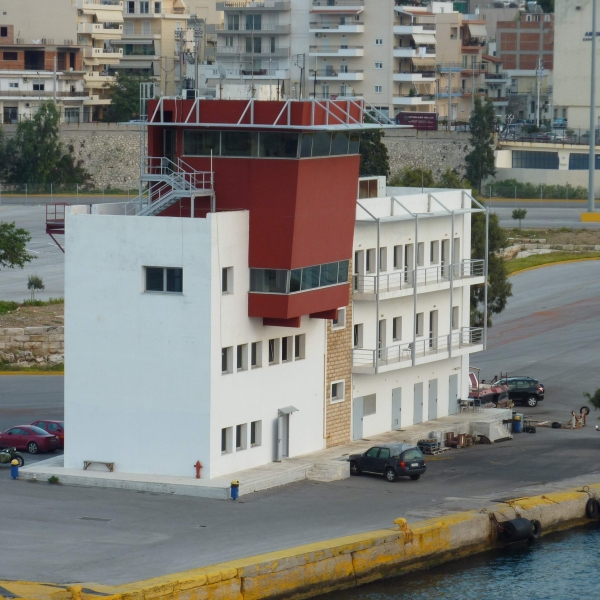
\includegraphics[scale=0.4]{images/le-piree.png}
\includegraphics[scale=0.4]{images/le-piree_lsd.png}
\end{center}

%-------------------------------------------------------------------------------
\section{Video}

This is an example of applying LSD, frame by frame, to a video:
\href{http://www.ipol.im/pub/algo/gjmr_line_segment_detector/data/algo/gjmr_line_segment_detector/video.mov}{original}(43Mb)
\href{http://www.ipol.im/pub/algo/gjmr_line_segment_detector/data/algo/gjmr_line_segment_detector/video.lsd.mp4}{lsd version}(62Mb).

%-------------------------------------------------------------------------------
\begin{thebibliography}{9}

  \bibitem{lsd} Rafael Grompone von Gioi, J\'er\'emie Jakubowicz,
  Jean-Michel Morel, Gregory Randall, \emph{LSD: A Fast Line Segment
  Detector with a False Detection Control}, IEEE Transactions on
  Pattern Analysis and Machine Intelligence, vol. 32, no. 4,
  pp. 722-732, April 2010.
  \url{http://doi.ieeecomputersociety.org/10.1109/TPAMI.2008.300}
  preprint: \url{http://www.cmla.ens-cachan.fr/fileadmin/Documentation/Prepublications/2008/CMLA2008-15.pdf}

   \bibitem{burns} J. Brian Burns, Allen R. Hanson, Edward
   M. Riseman, \emph{Extracting Straight Lines}, IEEE Transactions on
   Pattern Analysis and Machine Intelligence, vol. 8, no. 4,
   pp. 425-455, 1986.

   \bibitem{dmm2000} Agn\`es Desolneux, Lionel Moisan, Jean-Michel
   Morel, \emph{Meaningful Alignments}, International Journal of
   Computer Vision, vol. 40, no. 1, pp. 7-23, 2000.
   \url{(http://dx.doi.org/10.1023/A:1026593302236}
   preprint: \url{http://www.cmla.ens-cachan.fr/fileadmin/Documentation/Prepublications/1999/CMLA1999-11.ps.gz}

   \bibitem{dmm2008} Agn\`es Desolneux, Lionel Moisan, Jean-Michel
   Morel, \emph{From Gestalt Theory to Image Analysis, a Probabilistic
   Approach}, Springer 2008.

   \bibitem{multiseg} Rafael Grompone von Gioi, J\'er\'emie
   Jakubowicz, Jean-Michel Morel, Gregory Randall, \emph{On Straight
   Line Segment Detection}, Journal of Mathematical Imaging and
   Vision, vol. 32, no. 3, pp. 313-347, November 2008.
   \url{(http://dx.doi.org/10.1007/s10851-008-0102-5}
   preprint: \url{http://www.cmla.ens-cachan.fr/fileadmin/Documentation/Prepublications/2007/CMLA2007-09.pdf}

\end{thebibliography}

\end{document}
%-------------------------------------------------------------------------------
